\documentclass{standalone}
\usepackage{tikz}
\usetikzlibrary{patterns, positioning}

\begin{document}
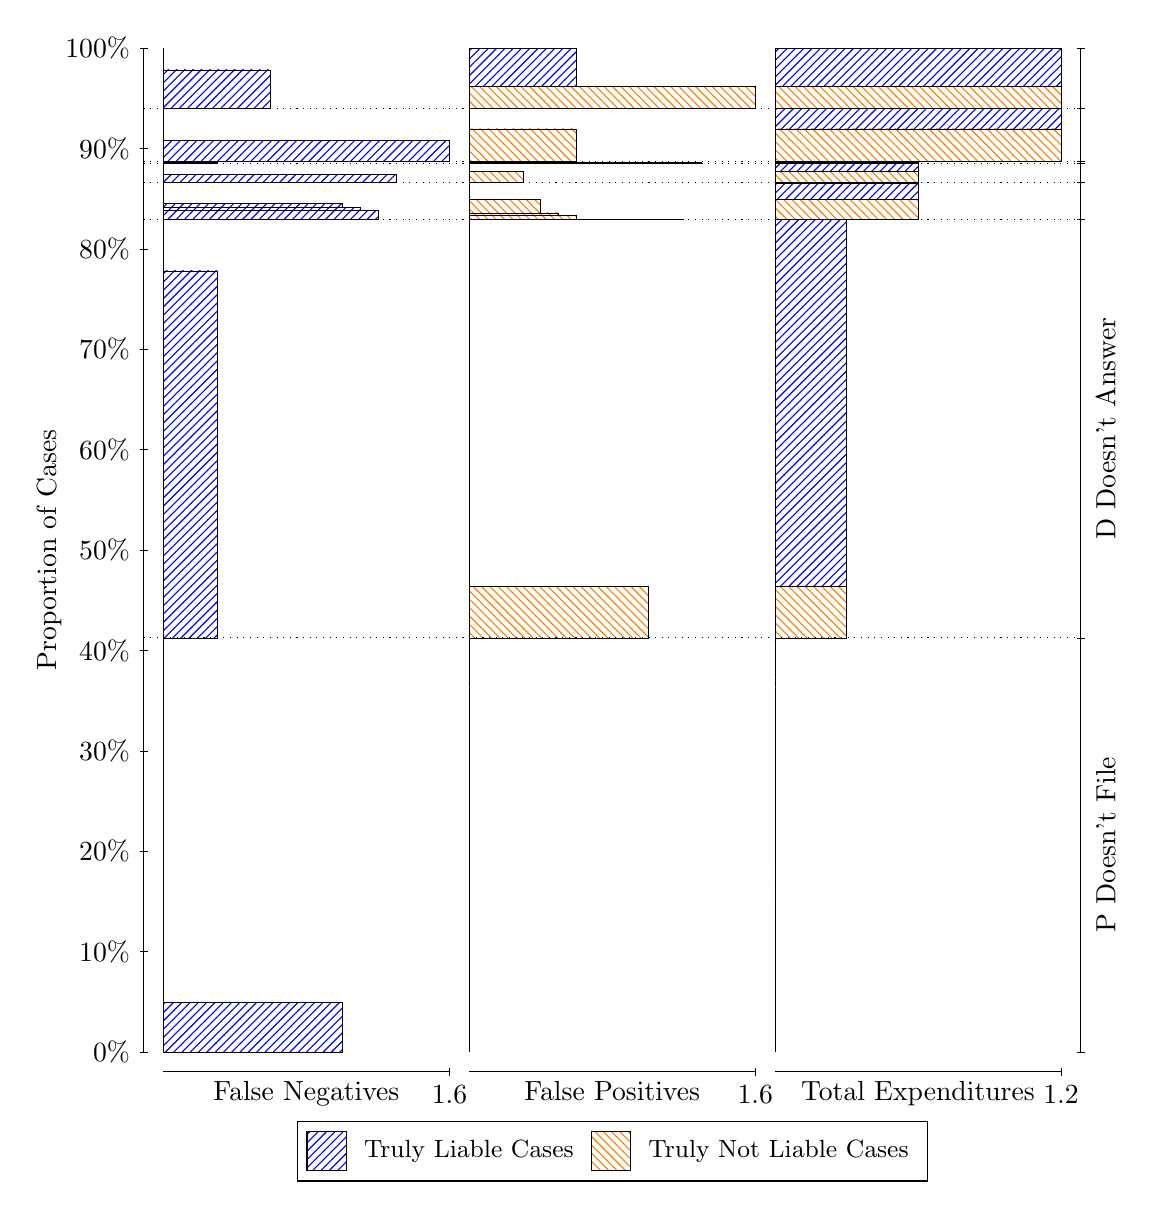
\begin{tikzpicture}
\draw[black, very thin] (1.5,1.75) -- (1.5,14.5);
\node[rotate=90, anchor=center] at (0.3, 8.125) {Proportion of Cases};
\draw[black, very thin] (1.45,1.75) -- (1.55,1.75);
\node[anchor=east] at (1.45, 1.75) {0\%};
\draw[black, very thin] (1.45,3.025) -- (1.55,3.025);
\node[anchor=east] at (1.45, 3.025) {10\%};
\draw[black, very thin] (1.45,4.3) -- (1.55,4.3);
\node[anchor=east] at (1.45, 4.3) {20\%};
\draw[black, very thin] (1.45,5.575) -- (1.55,5.575);
\node[anchor=east] at (1.45, 5.575) {30\%};
\draw[black, very thin] (1.45,6.85) -- (1.55,6.85);
\node[anchor=east] at (1.45, 6.85) {40\%};
\draw[black, very thin] (1.45,8.125) -- (1.55,8.125);
\node[anchor=east] at (1.45, 8.125) {50\%};
\draw[black, very thin] (1.45,9.4) -- (1.55,9.4);
\node[anchor=east] at (1.45, 9.4) {60\%};
\draw[black, very thin] (1.45,10.675) -- (1.55,10.675);
\node[anchor=east] at (1.45, 10.675) {70\%};
\draw[black, very thin] (1.45,11.95) -- (1.55,11.95);
\node[anchor=east] at (1.45, 11.95) {80\%};
\draw[black, very thin] (1.45,13.225) -- (1.55,13.225);
\node[anchor=east] at (1.45, 13.225) {90\%};
\draw[black, very thin] (1.45,14.5) -- (1.55,14.5);
\node[anchor=east] at (1.45, 14.5) {100\%};

\draw[black, very thin] (13.4,1.75) -- (13.4,14.5);
\draw[black, very thin] (13.35,1.75) -- (13.45,1.75);
\node[anchor=west] at (13.35, 1.75) {};
\draw[black, very thin] (13.35,7.01) -- (13.45,7.01);
\node[anchor=west] at (13.35, 7.01) {};
\draw[black, very thin] (13.35,12.32) -- (13.45,12.32);
\node[anchor=west] at (13.35, 12.32) {};
\draw[black, very thin] (13.35,12.789) -- (13.45,12.789);
\node[anchor=west] at (13.35, 12.789) {};
\draw[black, very thin] (13.35,13.032) -- (13.45,13.032);
\node[anchor=west] at (13.35, 13.032) {};
\draw[black, very thin] (13.35,13.064) -- (13.45,13.064);
\node[anchor=west] at (13.35, 13.064) {};
\draw[black, very thin] (13.35,13.736) -- (13.45,13.736);
\node[anchor=west] at (13.35, 13.736) {};
\draw[black, very thin] (13.35,14.5) -- (13.45,14.5);
\node[anchor=west] at (13.35, 14.5) {};

\draw[black, very thin, pattern color=blue, pattern=north east lines] (1.75,1.75) rectangle (4.0208,2.3828);
\draw[black, very thin, pattern color=orange, pattern=north west lines] (1.75,2.3828) rectangle (1.75,7.01);
\draw[black, very thin, pattern color=blue, pattern=north east lines] (1.75,7.01) rectangle (2.4312,11.669);
\draw[black, very thin, pattern color=orange, pattern=north west lines] (1.75,11.669) rectangle (1.75,12.32);
\draw[black, very thin, pattern color=blue, pattern=north east lines] (1.75,12.32) rectangle (4.475,12.442);
\draw[black, very thin, pattern color=blue, pattern=north east lines] (1.75,12.442) rectangle (4.2479,12.478);
\draw[black, very thin, pattern color=blue, pattern=north east lines] (1.75,12.478) rectangle (4.0208,12.524);
\draw[black, very thin, pattern color=blue, pattern=north east lines] (1.75,12.524) rectangle (3.7937,12.525);
\draw[black, very thin, pattern color=blue, pattern=north east lines] (1.75,12.525) rectangle (3.7937,12.525);
\draw[black, very thin, pattern color=blue, pattern=north east lines] (1.75,12.525) rectangle (3.5667,12.527);
\draw[black, very thin, pattern color=blue, pattern=north east lines] (1.75,12.527) rectangle (3.3396,12.528);
\draw[black, very thin, pattern color=blue, pattern=north east lines] (1.75,12.528) rectangle (3.1125,12.529);
\draw[black, very thin, pattern color=blue, pattern=north east lines] (1.75,12.529) rectangle (2.8854,12.529);
\draw[black, very thin, pattern color=blue, pattern=north east lines] (1.75,12.529) rectangle (2.6583,12.531);
\draw[black, very thin, pattern color=orange, pattern=north west lines] (1.75,12.531) rectangle (1.75,12.789);
\draw[black, very thin, pattern color=blue, pattern=north east lines] (1.75,12.789) rectangle (4.7021,12.891);
\draw[black, very thin, pattern color=orange, pattern=north west lines] (1.75,12.891) rectangle (1.75,13.032);
\draw[black, very thin, pattern color=blue, pattern=north east lines] (1.75,13.032) rectangle (2.4312,13.051);
\draw[black, very thin, pattern color=orange, pattern=north west lines] (1.75,13.051) rectangle (1.75,13.064);
\draw[black, very thin, pattern color=blue, pattern=north east lines] (1.75,13.064) rectangle (5.3833,13.329);
\draw[black, very thin, pattern color=orange, pattern=north west lines] (1.75,13.329) rectangle (1.75,13.736);
\draw[black, very thin, pattern color=blue, pattern=north east lines] (1.75,13.736) rectangle (3.1125,14.221);
\draw[black, very thin, pattern color=orange, pattern=north west lines] (1.75,14.221) rectangle (1.75,14.5);
\draw[black, very thin, pattern color=orange, pattern=north west lines] (5.6333,1.75) rectangle (5.6333,6.3773);
\draw[black, very thin, pattern color=blue, pattern=north east lines] (5.6333,6.3773) rectangle (5.6333,7.01);
\draw[black, very thin, pattern color=orange, pattern=north west lines] (5.6333,7.01) rectangle (7.9042,7.6607);
\draw[black, very thin, pattern color=blue, pattern=north east lines] (5.6333,7.6607) rectangle (5.6333,12.32);
\draw[black, very thin, pattern color=orange, pattern=north west lines] (5.6333,12.32) rectangle (8.3583,12.321);
\draw[black, very thin, pattern color=orange, pattern=north west lines] (5.6333,12.321) rectangle (8.1313,12.322);
\draw[black, very thin, pattern color=orange, pattern=north west lines] (5.6333,12.322) rectangle (7.9042,12.322);
\draw[black, very thin, pattern color=orange, pattern=north west lines] (5.6333,12.322) rectangle (7.6771,12.323);
\draw[black, very thin, pattern color=orange, pattern=north west lines] (5.6333,12.323) rectangle (7.45,12.325);
\draw[black, very thin, pattern color=orange, pattern=north west lines] (5.6333,12.325) rectangle (7.2229,12.326);
\draw[black, very thin, pattern color=orange, pattern=north west lines] (5.6333,12.326) rectangle (6.9958,12.37);
\draw[black, very thin, pattern color=orange, pattern=north west lines] (5.6333,12.37) rectangle (6.7687,12.406);
\draw[black, very thin, pattern color=orange, pattern=north west lines] (5.6333,12.406) rectangle (6.5417,12.578);
\draw[black, very thin, pattern color=blue, pattern=north east lines] (5.6333,12.578) rectangle (6.0875,12.58);
\draw[black, very thin, pattern color=blue, pattern=north east lines] (5.6333,12.58) rectangle (5.8604,12.58);
\draw[black, very thin, pattern color=blue, pattern=north east lines] (5.6333,12.58) rectangle (5.6333,12.789);
\draw[black, very thin, pattern color=orange, pattern=north west lines] (5.6333,12.789) rectangle (6.3146,12.929);
\draw[black, very thin, pattern color=blue, pattern=north east lines] (5.6333,12.929) rectangle (5.6333,13.032);
\draw[black, very thin, pattern color=orange, pattern=north west lines] (5.6333,13.032) rectangle (8.5854,13.045);
\draw[black, very thin, pattern color=blue, pattern=north east lines] (5.6333,13.045) rectangle (6.3146,13.064);
\draw[black, very thin, pattern color=orange, pattern=north west lines] (5.6333,13.064) rectangle (6.9958,13.472);
\draw[black, very thin, pattern color=blue, pattern=north east lines] (5.6333,13.472) rectangle (5.6333,13.736);
\draw[black, very thin, pattern color=orange, pattern=north west lines] (5.6333,13.736) rectangle (9.2667,14.015);
\draw[black, very thin, pattern color=blue, pattern=north east lines] (5.6333,14.015) rectangle (6.9958,14.5);
\draw[black, very thin, pattern color=orange, pattern=north west lines] (9.5167,1.75) rectangle (9.5167,6.3773);
\draw[black, very thin, pattern color=blue, pattern=north east lines] (9.5167,6.3773) rectangle (9.5167,7.01);
\draw[black, very thin, pattern color=orange, pattern=north west lines] (9.5167,7.01) rectangle (10.425,7.6607);
\draw[black, very thin, pattern color=blue, pattern=north east lines] (9.5167,7.6607) rectangle (10.425,12.32);
\draw[black, very thin, pattern color=orange, pattern=north west lines] (9.5167,12.32) rectangle (11.333,12.323);
\draw[black, very thin, pattern color=blue, pattern=north east lines] (9.5167,12.323) rectangle (11.333,12.326);
\draw[black, very thin, pattern color=orange, pattern=north west lines] (9.5167,12.326) rectangle (11.333,12.579);
\draw[black, very thin, pattern color=blue, pattern=north east lines] (9.5167,12.579) rectangle (11.333,12.783);
\draw[black, very thin, pattern color=orange, pattern=north west lines] (9.5167,12.783) rectangle (11.333,12.786);
\draw[black, very thin, pattern color=blue, pattern=north east lines] (9.5167,12.786) rectangle (11.333,12.789);
\draw[black, very thin, pattern color=orange, pattern=north west lines] (9.5167,12.789) rectangle (11.333,12.929);
\draw[black, very thin, pattern color=blue, pattern=north east lines] (9.5167,12.929) rectangle (11.333,13.032);
\draw[black, very thin, pattern color=orange, pattern=north west lines] (9.5167,13.032) rectangle (11.333,13.045);
\draw[black, very thin, pattern color=blue, pattern=north east lines] (9.5167,13.045) rectangle (11.333,13.064);
\draw[black, very thin, pattern color=orange, pattern=north west lines] (9.5167,13.064) rectangle (13.15,13.472);
\draw[black, very thin, pattern color=blue, pattern=north east lines] (9.5167,13.472) rectangle (13.15,13.736);
\draw[black, very thin, pattern color=orange, pattern=north west lines] (9.5167,13.736) rectangle (13.15,14.015);
\draw[black, very thin, pattern color=blue, pattern=north east lines] (9.5167,14.015) rectangle (13.15,14.5);
\draw[black, dotted] (1.5,7.01) -- (13.4,7.01);
\draw[black, dotted] (1.5,12.32) -- (13.4,12.32);
\draw[black, dotted] (1.5,12.789) -- (13.4,12.789);
\draw[black, dotted] (1.5,13.032) -- (13.4,13.032);
\draw[black, dotted] (1.5,13.064) -- (13.4,13.064);
\draw[black, dotted] (1.5,13.736) -- (13.4,13.736);
\draw[black, very thin] (1.75,1.5) -- (5.3833,1.5);
\node[anchor=north] at (3.5667, 1.5) {False Negatives};
\draw[black, very thin] (5.3833,1.45) -- (5.3833,1.55);
\node[anchor=north] at (5.3833, 1.45) {1.6};

\draw[black, very thin] (5.6333,1.5) -- (9.2667,1.5);
\node[anchor=north] at (7.45, 1.5) {False Positives};
\draw[black, very thin] (9.2667,1.45) -- (9.2667,1.55);
\node[anchor=north] at (9.2667, 1.45) {1.6};

\draw[black, very thin] (9.5167,1.5) -- (13.15,1.5);
\node[anchor=north] at (11.333, 1.5) {Total Expenditures};
\draw[black, very thin] (13.15,1.45) -- (13.15,1.55);
\node[anchor=north] at (13.15, 1.45) {1.2};

\node[black, centered, rotate=90] at (13.72, 4.38) {P Doesn't File};
\node[black, centered, rotate=90] at (13.72, 9.665) {D Doesn't Answer};






\draw (7.449999999999999,1.5) node[draw=none] (baseCoordinate) {};
\begin{scope}[align=center]
        \matrix[scale=0.5, draw=black, below=0.5cm of baseCoordinate, nodes={draw}, column sep=0.1cm]{
            \node[rectangle, draw, minimum width=0.5cm, minimum height=0.5cm, pattern=north east lines, pattern color=blue] {}; &
            \node[draw=none, font=\small] (B) {Truly Liable Cases}; &
            \node[rectangle, draw, minimum width=0.5cm, minimum height=0.5cm, pattern=north west lines, pattern color=orange] {}; &
            \node[draw=none, font=\small] (B) {Truly Not Liable Cases}; \\
            };
\end{scope}

\end{tikzpicture}
\end{document}